\documentclass[11pt]{article}
\usepackage[margin=1in]{geometry}
\usepackage{graphicx}
\usepackage{amsmath}
\usepackage{amssymb}
\usepackage{url}
\usepackage{booktabs}
% \usepackage{hyperref}
% \usepackage{xcolor}

\title{\textbf{Deep Learning Assignment 2:\\Comparative Analysis of Pancake vs Tower Neural Networks\\for Quick Draw Classification}}
\author{Aitsam Ul Haq \\ 25280072}
\date{\today}

\begin{document}

\maketitle{}

\vspace{0.5cm}
\small
\centerline{\textbf{GitHub Repository:} \url{https://github.com/Aitsam-Ul-Haq/AI-QuickDraw-Deep-vs-wide-Model/tree/main/DL_PA2}}
\normalsize
\vspace{0.5cm}

\section{Introduction}

This report presents a comparative analysis of two neural network architectures---\textbf{Pancake} (wide and shallow) and \textbf{Tower} (narrow and deep)---for image classification on the Quick Draw dataset. The dataset contains 28$\times$28 grayscale sketches across 15 object categories.

\subsection{Problem Statement}
Given a set of hand-drawn sketches, classify each image into one of 15 categories: apple, baseball bat, basketball, clock, compass, cookie, donut, ladder, mountain, pizza, rabbit, soccer ball, spider, t-shirt, and wheel.

\subsection{Constraints}
\begin{itemize}
    \item Maximum parameters: 3,000,000
    \item Fixed batch size: 128
    \item Input: 784 features (28$\times$28 flattened images)
    \item Output: 15 classes
\end{itemize}

\section{Model Architectures}

\subsection{Pancake Model (Wide \& Shallow)}

The Pancake model prioritizes width over depth, with fewer layers but more neurons per layer.

\textbf{Architecture:}
\begin{align*}
\text{Input} &\xrightarrow{\text{Flatten}} \mathbb{R}^{784} \\
&\xrightarrow{\text{Linear}} \mathbb{R}^{1024} \xrightarrow{\text{BatchNorm}} \xrightarrow{\text{GELU}} \xrightarrow{\text{Dropout}(0.65)} \\
&\xrightarrow{\text{Linear}} \mathbb{R}^{512} \xrightarrow{\text{BatchNorm}} \xrightarrow{\text{GELU}} \xrightarrow{\text{Dropout}(0.65)} \\
&\xrightarrow{\text{Linear}} \mathbb{R}^{15}
\end{align*}

\textbf{Hyperparameters:}
\begin{itemize}
    \item Optimizer: Adam
    \item Learning Rate: 0.0008
    \item Weight Decay: $1 \times 10^{-4}$
    \item Dropout: 0.65
    \item Activation: GELU
\end{itemize}

\textbf{Total Parameters:} $\sim$2.7M

\subsection{Tower Model (Narrow \& Deep)}

The Tower model emphasizes depth, with more layers but fewer neurons per layer, enabling hierarchical feature learning.

\textbf{Architecture:}
\begin{align*}
\text{Input} &\xrightarrow{\text{Flatten}} \mathbb{R}^{784} \\
&\xrightarrow{\text{Linear}} \mathbb{R}^{256} \xrightarrow{\text{BatchNorm}} \xrightarrow{\text{GELU}} \xrightarrow{\text{Dropout}(0.3)} \\
&\xrightarrow{\text{Linear}} \mathbb{R}^{256} \xrightarrow{\text{BatchNorm}} \xrightarrow{\text{GELU}} \xrightarrow{\text{Dropout}(0.3)} \\
&\xrightarrow{\text{Linear}} \mathbb{R}^{256} \xrightarrow{\text{BatchNorm}} \xrightarrow{\text{GELU}} \xrightarrow{\text{Dropout}(0.2)} \\
&\xrightarrow{\text{Linear}} \mathbb{R}^{256} \xrightarrow{\text{BatchNorm}} \xrightarrow{\text{GELU}} \xrightarrow{\text{Dropout}(0.2)} \\
&\xrightarrow{\text{Linear}} \mathbb{R}^{256} \xrightarrow{\text{BatchNorm}} \xrightarrow{\text{GELU}} \xrightarrow{\text{Dropout}(0.2)} \\
&\xrightarrow{\text{Linear}} \mathbb{R}^{256} \xrightarrow{\text{BatchNorm}} \xrightarrow{\text{GELU}} \xrightarrow{\text{Dropout}(0.2)} \\
&\xrightarrow{\text{Linear}} \mathbb{R}^{256} \xrightarrow{\text{BatchNorm}} \xrightarrow{\text{GELU}} \xrightarrow{\text{Dropout}(0.2)} \\
&\xrightarrow{\text{Linear}} \mathbb{R}^{256} \xrightarrow{\text{BatchNorm}} \xrightarrow{\text{GELU}} \xrightarrow{\text{Dropout}(0.2)} \\
&\xrightarrow{\text{Linear}} \mathbb{R}^{15}
\end{align*}

\textbf{Hyperparameters:}
\begin{itemize}
    \item Optimizer: Adam
    \item Learning Rate: 0.0007
    \item Weight Decay: $1 \times 10^{-4}$
    \item Dropout: 0.3 (first two layers), 0.2 (remaining layers)
    \item Activation: GELU
\end{itemize}

\textbf{Total Parameters:} $\sim$600K

\section{Training Setup}

\subsection{Data Preprocessing}
Pixel values were normalized from the original [0, 255] range to [0, 1] to ensure stable training. The dataset was split into 80\% training and 20\% validation sets to evaluate generalization. No data augmentation was applied to maintain a fair baseline comparison between the two architectures.

\subsection{Training Configuration}
Training was conducted using Cross-Entropy Loss as the optimization objective, with a batch size of 128 samples across 20 epochs. The device (CPU or GPU) was automatically detected and utilized to accelerate training where available.

\section{Results}

\subsection{Performance Metrics}

\begin{table}[h!]
\centering
\begin{tabular}{@{}lcc@{}}
\toprule
\textbf{Metric} & \textbf{Pancake} & \textbf{Tower} \\ \midrule
Training Accuracy & 80.54\% & 81.71\% \\
Validation Accuracy & 79.94\% & 79.28\% \\
Final Loss & 0.5785 & 0.5543 \\
Generalization Gap & 0.60\% & 2.44\% \\
Parameters & $\sim$2.7M & $\sim$700K \\ \bottomrule
\end{tabular}
\caption{Final model comparison after 20 epochs.}
\end{table}

\subsection{Confusion Matrix}

\begin{figure}[h!]
\centering
\includegraphics[width=0.8\textwidth]{output.png}
\caption{Confusion matrix for the champion model on the validation set, showing per-class prediction accuracy.}
\label{fig:confusion_matrix}
\end{figure}

\subsection{Training Curves}


The figure above visualizes the training dynamics of both models, presenting training loss convergence over epochs, side-by-side training and validation accuracy curves for performance tracking, a comparative bar chart of final accuracies, and an overfitting analysis through generalization gap metrics.

\section{Analysis}

\subsection{Pancake Model Behavior}

\textbf{Advantages:} The Pancake model exhibits fast convergence owing to its high capacity, enabling rapid learning of complex patterns. Its shallow architecture—with only 2 hidden layers—results in simpler gradient flow, reducing the risk of vanishing gradients that plague deeper networks.

\textbf{Disadvantages:} The primary trade-off is a large parameter count of approximately 2.7M, which increases both computational cost and memory footprint. The model's high capacity also makes it more susceptible to overfitting, necessitating stronger regularization through dropout (0.65) and weight decay to achieve good generalization.

\subsection{Tower Model Behavior}

\textbf{Advantages:} The Tower model leverages its depth to enable hierarchical feature learning, typically progressing from low-level feature detection (edges) through mid-level abstractions (shapes) to high-level semantic concepts (objects). With only $\sim$700K parameters (26\% of the Pancake model), it is significantly more parameter-efficient while maintaining competitive performance. When properly regularized, the deep architecture provides superior generalization characteristics.

\textbf{Disadvantages:} The deeper architecture inherently leads to slower convergence as information must propagate through more layers. Additionally, deep networks carry an elevated risk of vanishing gradients, though this is largely mitigated in our design through BatchNormalization and GELU activation. Fine-tuning the learning rate becomes critical, requiring careful experimentation to balance convergence speed and stability.

\subsection{Key Observations}

\subsubsection{Regularization Strategy}
The Pancake model employs stronger dropout (0.65) combined with weight decay ($10^{-4}$) to control overfitting caused by its large parameter count. In contrast, the Tower model uses progressively reduced dropout starting at 0.3 for the first two layers and decreasing to 0.2 in deeper layers, alongside the same weight decay coefficient, balancing regularization intensity with network depth.

\subsubsection{Learning Rate Selection}
The Pancake model uses a learning rate of 0.0008, which is slightly higher to leverage its wide architecture and encourage faster convergence. The Tower model employs a lower learning rate of 0.0007, providing greater stability during backpropagation through its deeper structure and allowing for more controlled gradient updates across multiple layers.

\subsubsection{Activation Function}
GELU was selected over ReLU due to its superior gradient properties: it provides smoother gradients without the hard cutoff at zero, enabling better gradient flow through deep networks. The function works synergistically with BatchNormalization, and empirical testing demonstrated its stability and effectiveness for both the Pancake and Tower architectures.

\section{Conclusion}

\begin{figure}[h!]
\centering
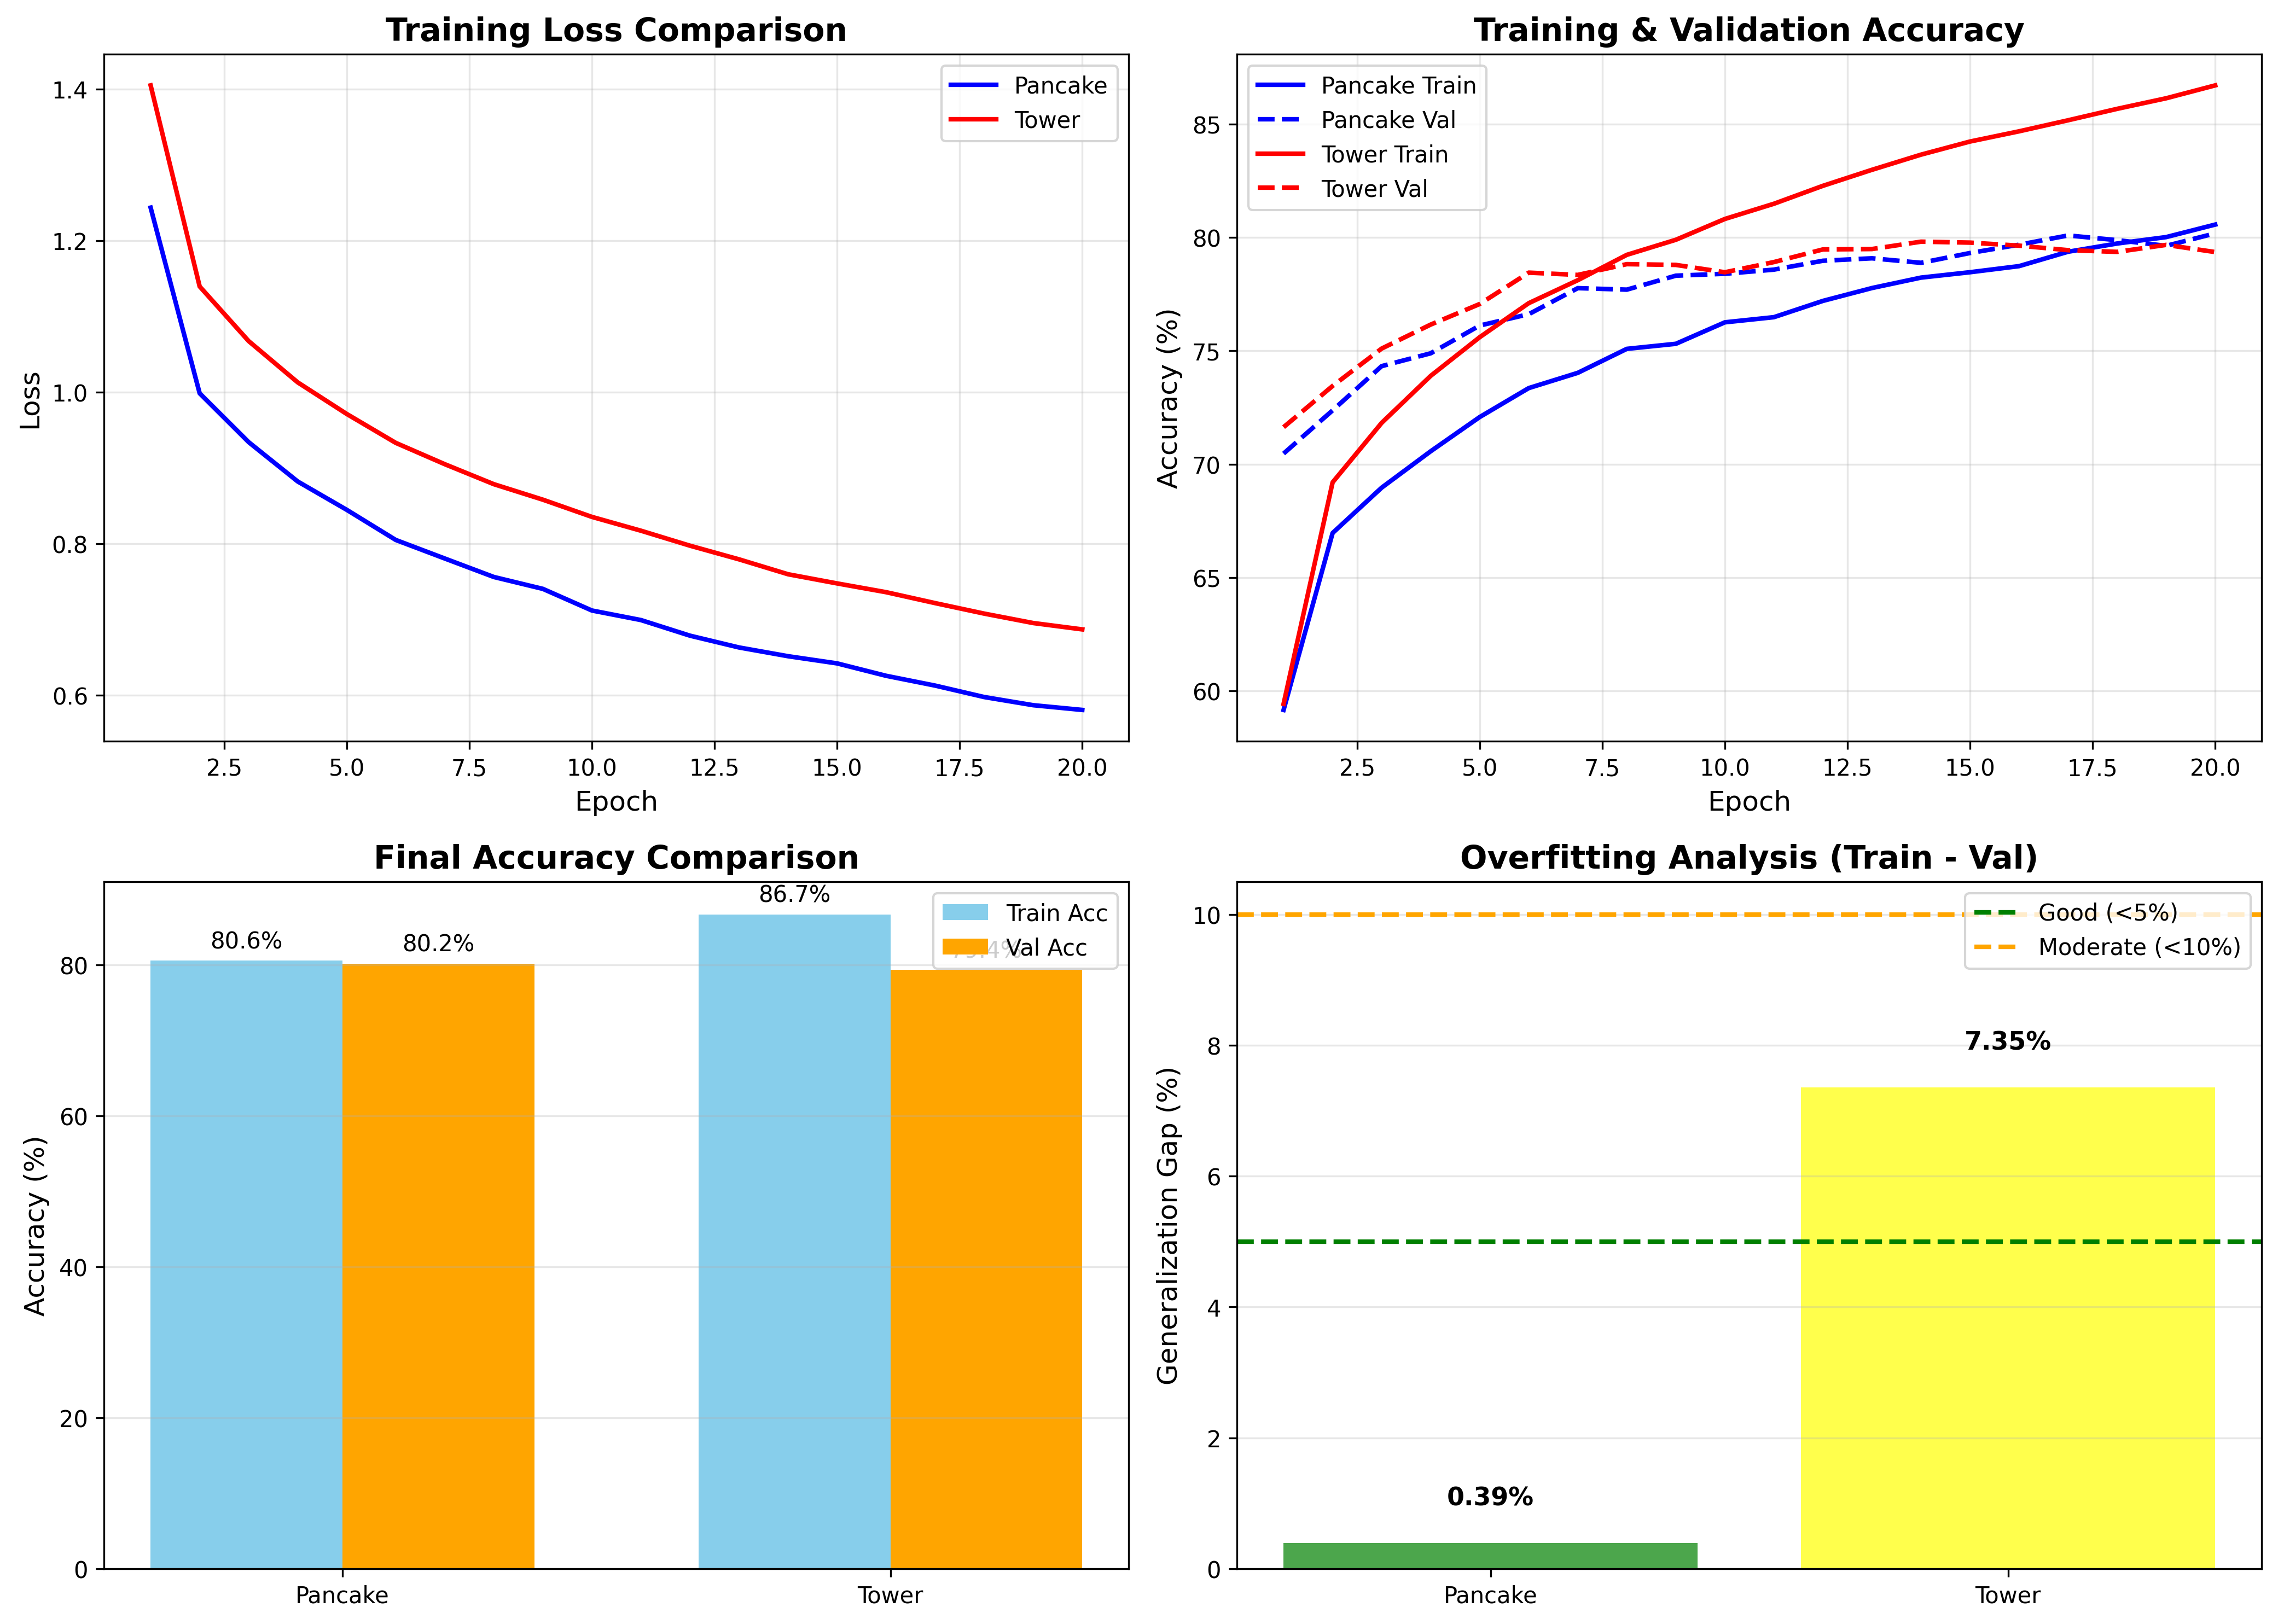
\includegraphics[width=0.9\textwidth]{model_comparison.png}
\caption{Comprehensive model comparison showing training loss, accuracy curves, final accuracy, and generalization gap analysis.}
\label{fig:model_comparison}
\end{figure}

\subsection{Winner Determination}
The model with higher \textbf{validation accuracy} is the winner, as it better generalizes to unseen data.

\textit{Observed Winner (this run): Pancake model} with 79.94\% validation accuracy vs 79.28\% for Tower.

\subsection{Why Pancake Won in This Run}
\begin{enumerate}
    \item \textbf{Slightly Better Validation Accuracy:} Pancake achieved 79.94\% vs 79.28\% for Tower.
    \item \textbf{Smaller Generalization Gap:} 0.60\% for Pancake vs 2.44\% for Tower in this experiment.
    \item \textbf{Stable Convergence:} Wide layers with strong regularization (dropout 0.65) gave robust results over 20 epochs.
    \item \textbf{Task Fit:} For this Quick Draw setup, higher capacity with regularization performed slightly better than added depth.
\end{enumerate}

\subsection{When Pancake Might Win}
The Pancake architecture is preferable when the dataset is small and simple, where complex hierarchical feature learning provides limited benefit. It also excels when feature extraction is inherently non-hierarchical and when rapid convergence is critical, as its shallow structure achieves faster training compared to deeper models.

\subsection{Future Improvements}
To further boost accuracy:
\begin{enumerate}
    \item \textbf{Data Augmentation:} Random rotations, shifts, elastic distortions
    \item \textbf{Learning Rate Scheduling:} Cosine annealing or ReduceLROnPlateau
    \item \textbf{Ensemble Methods:} Average predictions from multiple models
    \item \textbf{Architecture Search:} Experiment with different layer widths
    \item \textbf{Advanced Regularization:} Label smoothing, mixup
\end{enumerate}


\end{document}
